


\begin{figure}[t!]
    \centering
  %\begin{subfigure}{7cm}
   % \centering
    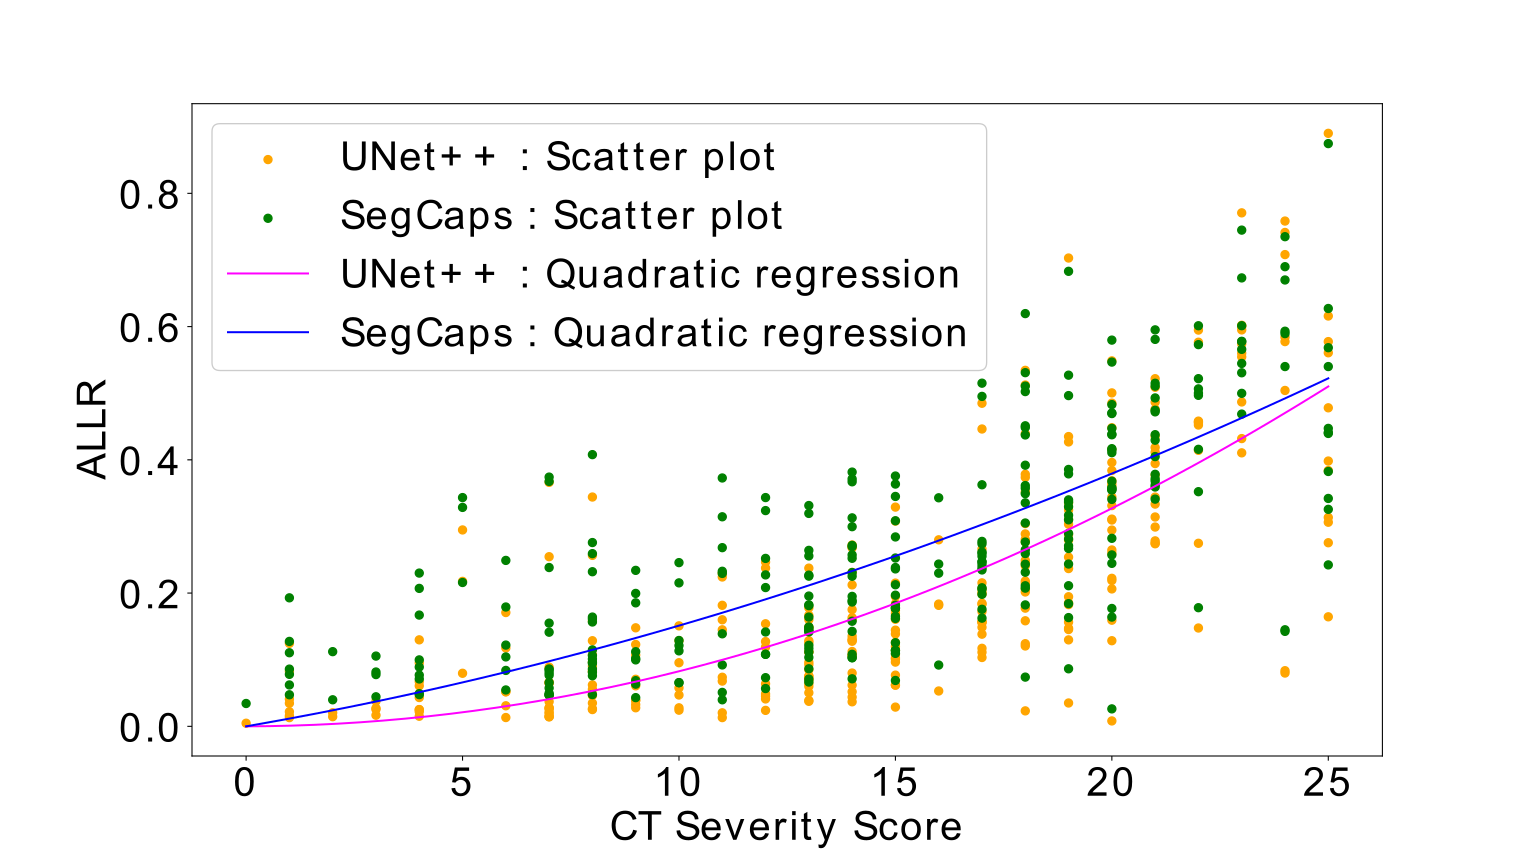
\includegraphics[width=\columnwidth]{images/Quadratic-Regression_1.png}
    %\\
     %\end{subfigure}
\caption{Scatter plots of ALLR (computed by UNet++ and SegCaps) versus CT severity score, and corresponding quadratic regression curve.}
\label{fig:RelationshipGraph}
\end{figure}

\begin{figure}[t!]
    \centering
  %\begin{subfigure}{7cm}
  %  \centering
    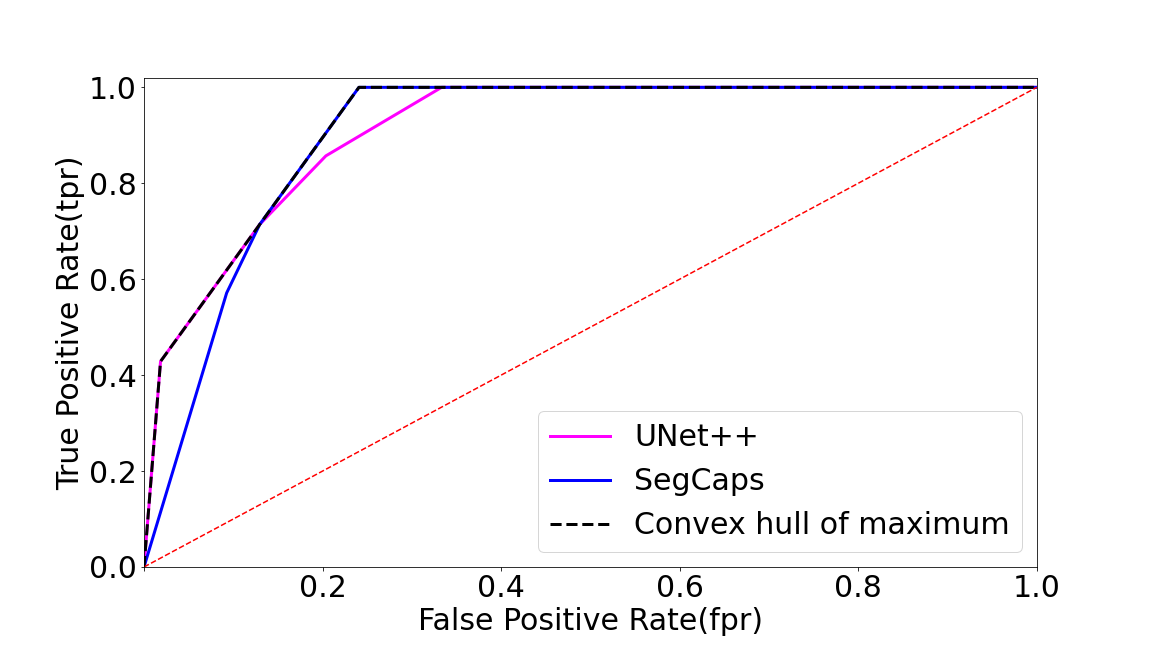
\includegraphics[width=1.0\columnwidth]{images/ROC-Overlay-fpr-tpr.png}
   % \\
% \end{subfigure}
\caption{Median ROC curves obtained by UNet++ (AUC: 0.912) and SegCaps (AUC: 0.904), as well as the convex hull of the maximum (AUC: 0.921).}
\label{fig:ROC_CUrve}
\end{figure}


\section{Experimental Results}

We begin by depicting representative CT scans, and corresponding lung segmentation and inflammation segmentation by UNet++ and SegCaps in Figs. \ref{Fig : Main Results}(a), \ref{Fig : Main Results}(b), \ref{Fig : Main Results}(c) and \ref{Fig : Main Results}(d), respectively. The results of inflammation segmentation present perceptible differences. Experts felt that UNet++ and SegCaps were slightly superior in segmenting consolidation and GGOs, respectively. However, statistically, their performances in terms of DC were nearly indistinguishable, as seen in Table \ref{tab:2d-IS}. However, this may not indicate truly similar performance, because the chosen baseline, as alluded earlier, may not provide a reliable reference.



%The segmentation performance is evaluated using multiple metrics. First, the Dice coefficient is calculated for the test subset of covid-challenge-dataset. Second, ALLRs generated for the MGMCH dataset using the segmentation models is compared with the CT severity scores. Finally,  outcome prediction models for need for ventilation in this set of patients, each using lung inflammation quantification by the three methods in question are compared. 




%Dice coefficients (DCs) for both UNet++ and SegCaps models were nearly equal. The values of DCs were relatively low, and we investigated this further. We found that there was overestimation of the inflamed area in the Covid segmentation challenge dataset when we performed in-house annotation of lung segments (by a practicing senior radiologist) as shown in Fig. \ref{Fig : Radiologist comparison}. Therefore, during our we modified the annotations and took only the region which have high density of inflammation in the mask, it cause somewhat underestimation in the generated mask and that intuition was also confirmed by the radiologists and is shown .

%Some examples of results obtained after UNet++ segmentation and SegCaps segmentation on MGMCH data are given in Fig \ref{Fig : Main Results}.

Towards more reliable comparison, scatter plot of ALLRs based on UNet++ (as well as SegCaps) versus CT severity scores is presented in Fig. \ref{fig:RelationshipGraph}. We obtained the quadratic regression curve in each case, and the respective root mean squared errors of 0.118 and 0.121 for UNet++ and SegCaps models. For linear regression, which provided a worse fit, respective correlation coefficients were 0.70 and 0.68. By these measures too, UNet++ and SegCaps performed almost similarly.

However, as shown in Fig. \ref{fig:ROC_CUrve}, the median ROC curves for predicting the need for MV using ALLRs based on UNet++ and SegCaps were found to be significantly different. Specifically, UNet++ performs superior in the low-FPR regime, and SegCaps in the high-FPR regime. This phenomenon possibly corroborates the aforementioned subjective opinion regarding their performance difference in case of consolidation and GGOs. In any case, by choosing the better tool in each regime, one may operate at a performance level (in terms of AUC) higher than either can achieve.   



% The AUC stands for "Area under the ROC Curve" shown in fig \ref{fig:ROC_CUrve} has median of 0.912 and standard deviation of 0.059 for UNet++ model and median of 0.904 and standard deviation of 0.054 in case of SegCaps. The dashed line in the curve shown in fig \ref{fig:ROC_CUrve} represents the convex hull whose combined auc median is 0.921.

\section{Discussion}

Here, we treated various types of lung parenchymal changes as the same class.
Class-wise differentiation (possibly statistically) and inflammation quantification may produce a more accurate score for the overall degree of lung inflammation, reflecting lung pathophysiology better. This work potentially opens up an area of discussion for choosing the most appropriate tool for quantification of various lung pathologies, which can be put to precise clinical use if they can be made context specific. For example, if a radiologist sees a GGO specific disease in a particular CT scan, s/he may choose to use a tool that is more appropriate for GGO while quantifying the total area involved in the disease, and use a different tool for consolidation-predominant disease. 